\chapter{Resultados del trabajo, en formato SCL}
\label{app:resultados2-codigos-SCL}


\newpage
\vspace*{\fill}
	\begingroup
\section{ICD del regulador de velocidad (regulaci�n primaria)}
	\endgroup
\vspace*{\fill}
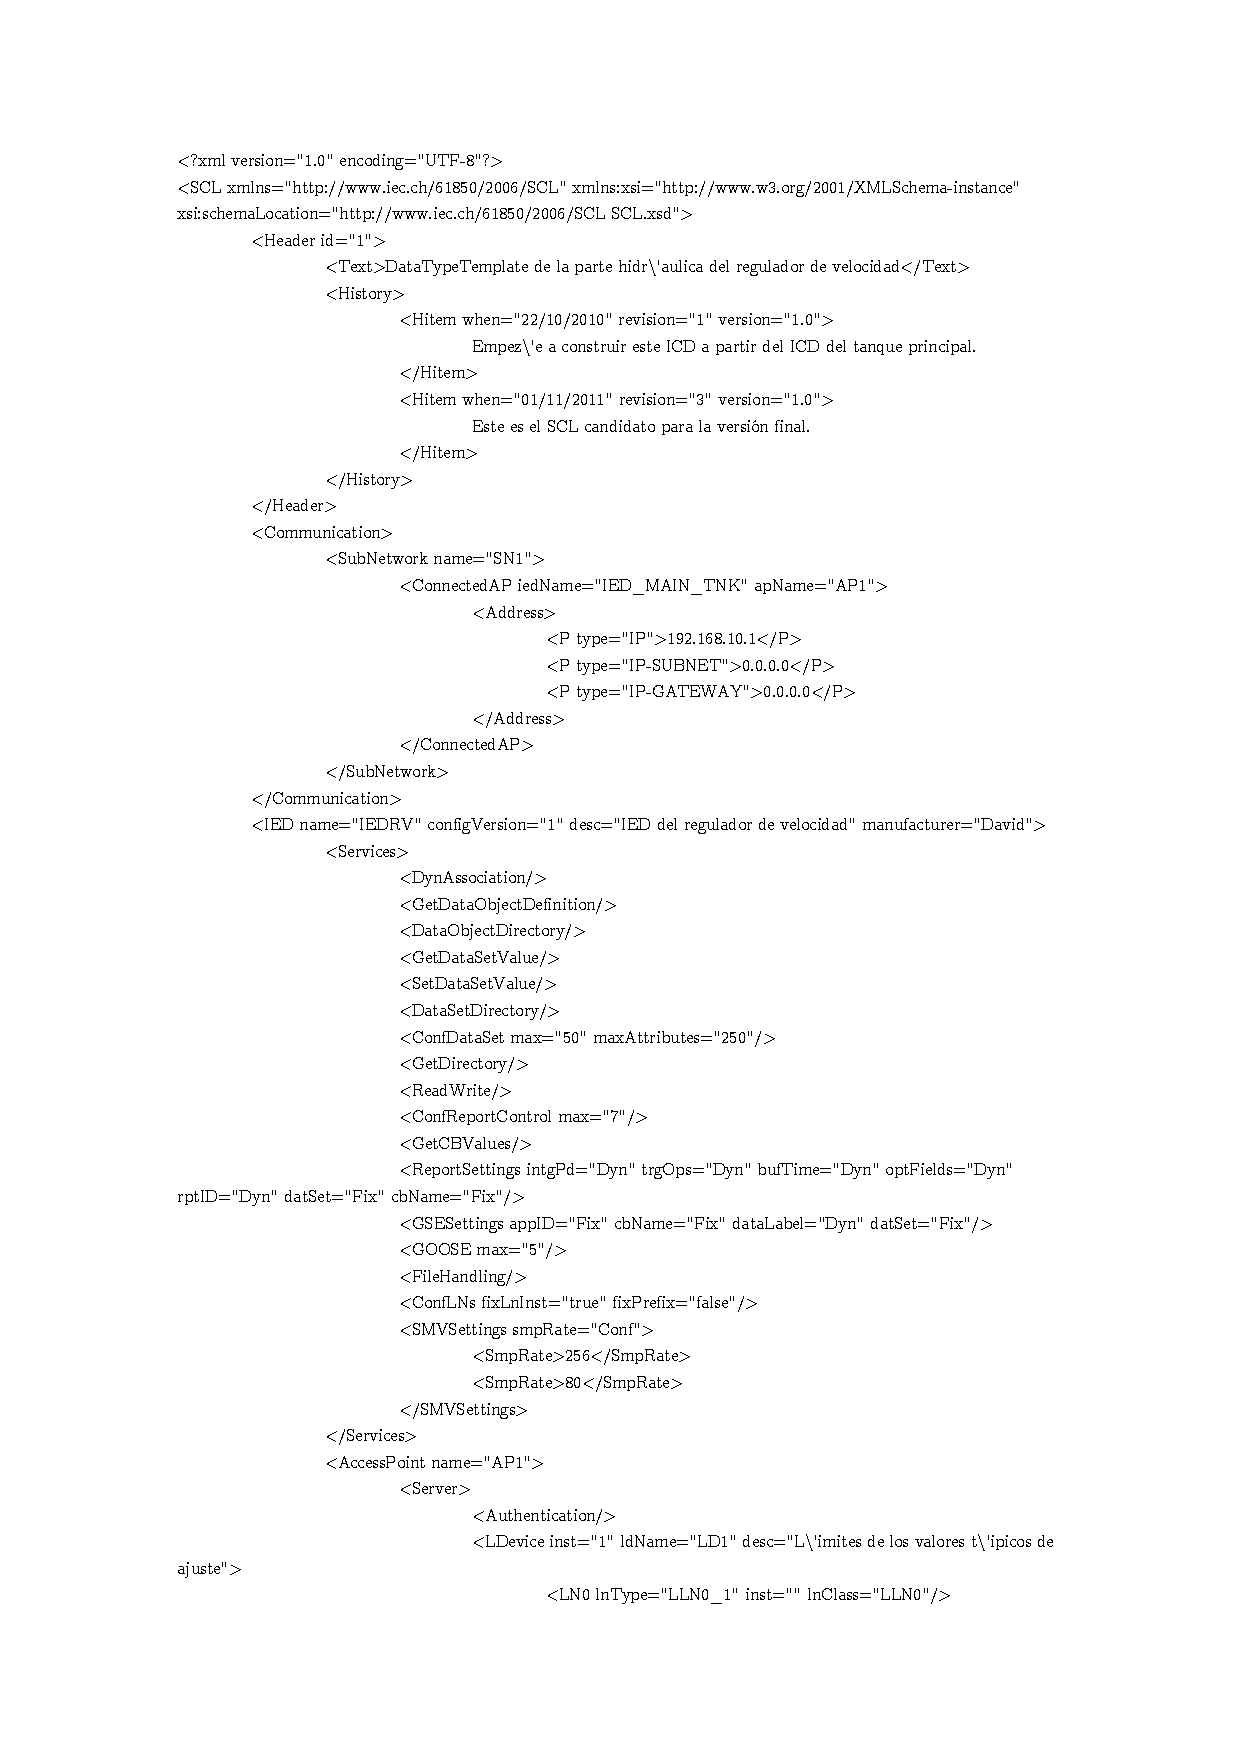
\includepdf[pages=1-4]{appendices/ICD-IED_RV.pdf} 
%\lstinputlisting[label=cod:ICD-IED_RV-primaria-xml,
%caption=ICD de la regulaci�n primaria]
%{governorModel/ICDs/IED_RV.xml} 



\vspace*{\fill}
	\begingroup
\section{ICD del regulador de velocidad (regulaci�n secundaria)}
	\endgroup
\vspace*{\fill}
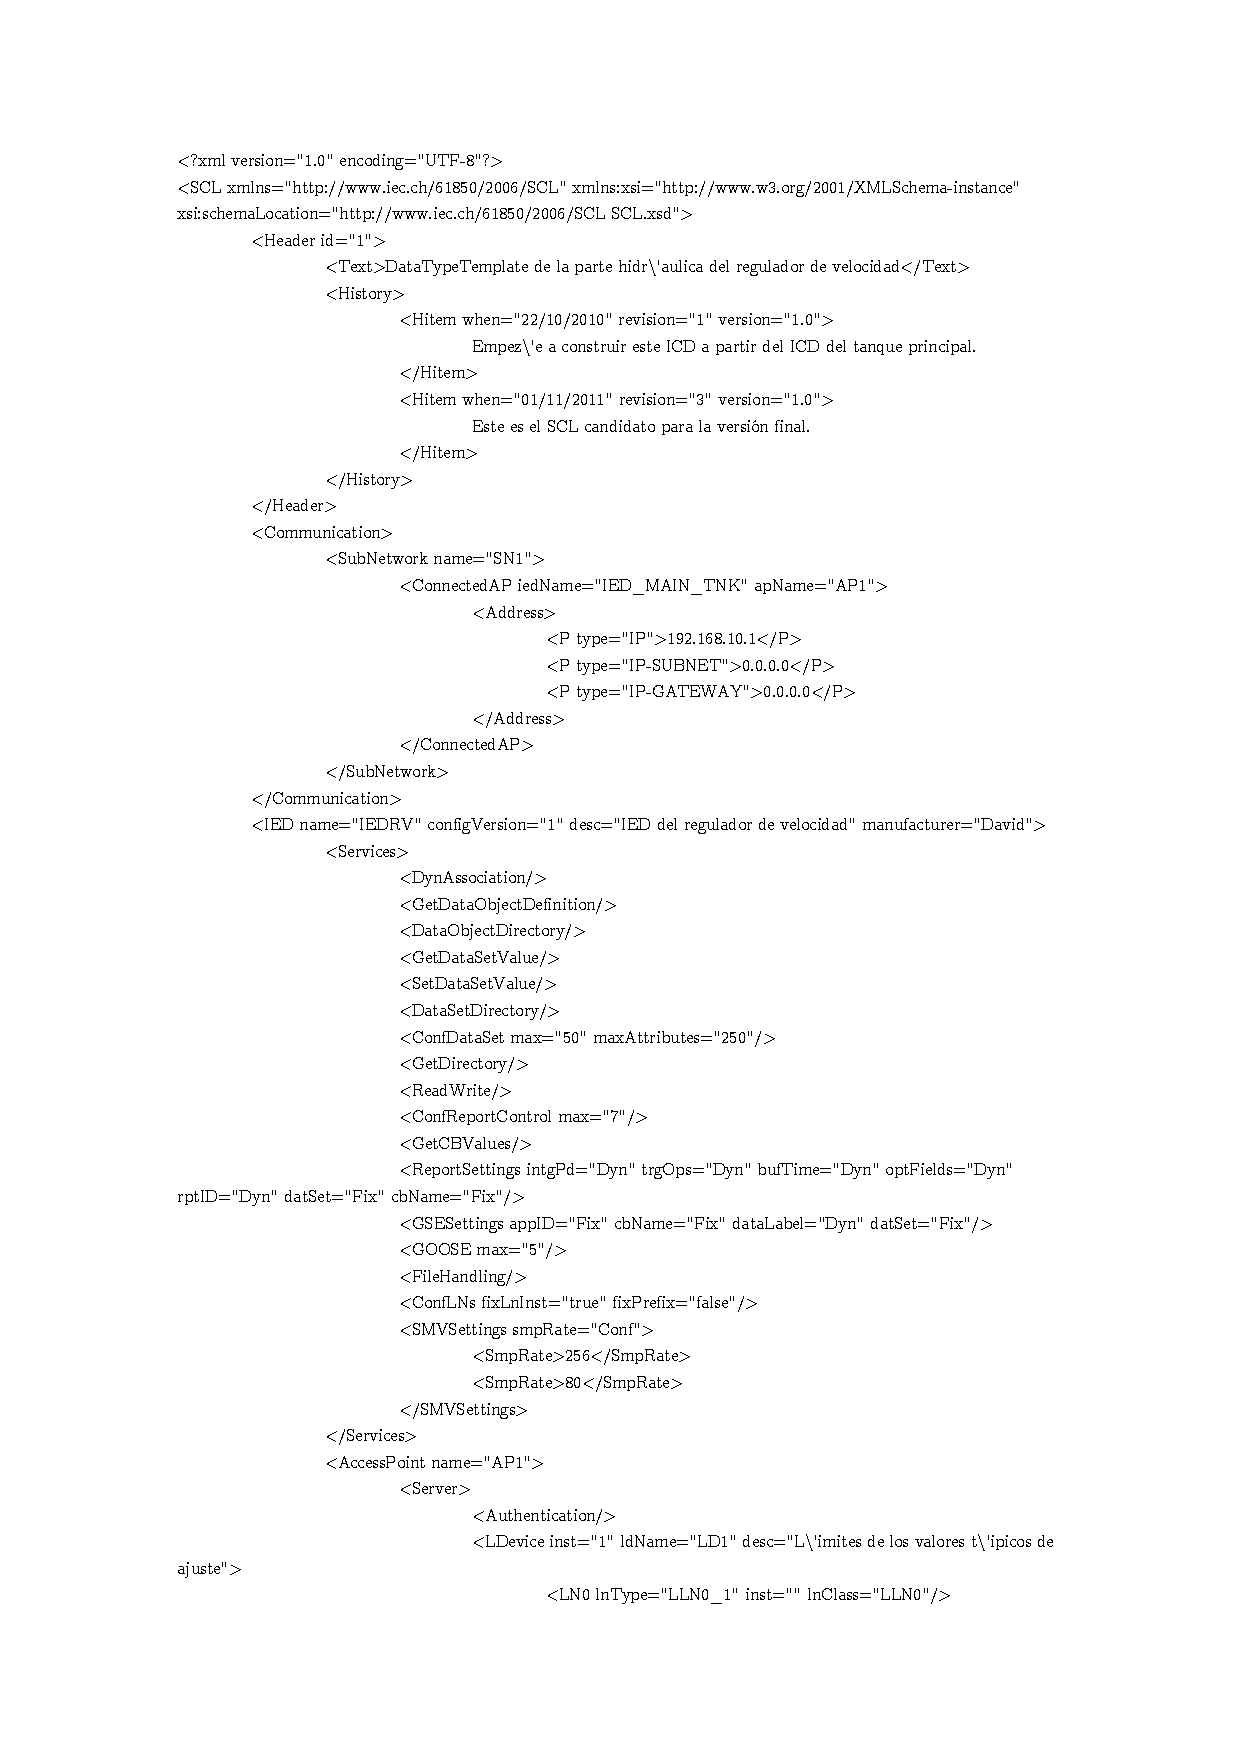
\includepdf[pages=1-4]{appendices/ICD-IED_RV.pdf} 


\vspace*{\fill}
	\begingroup
\section{ICD del sensor de rotaci�n}
	\endgroup
\vspace*{\fill}
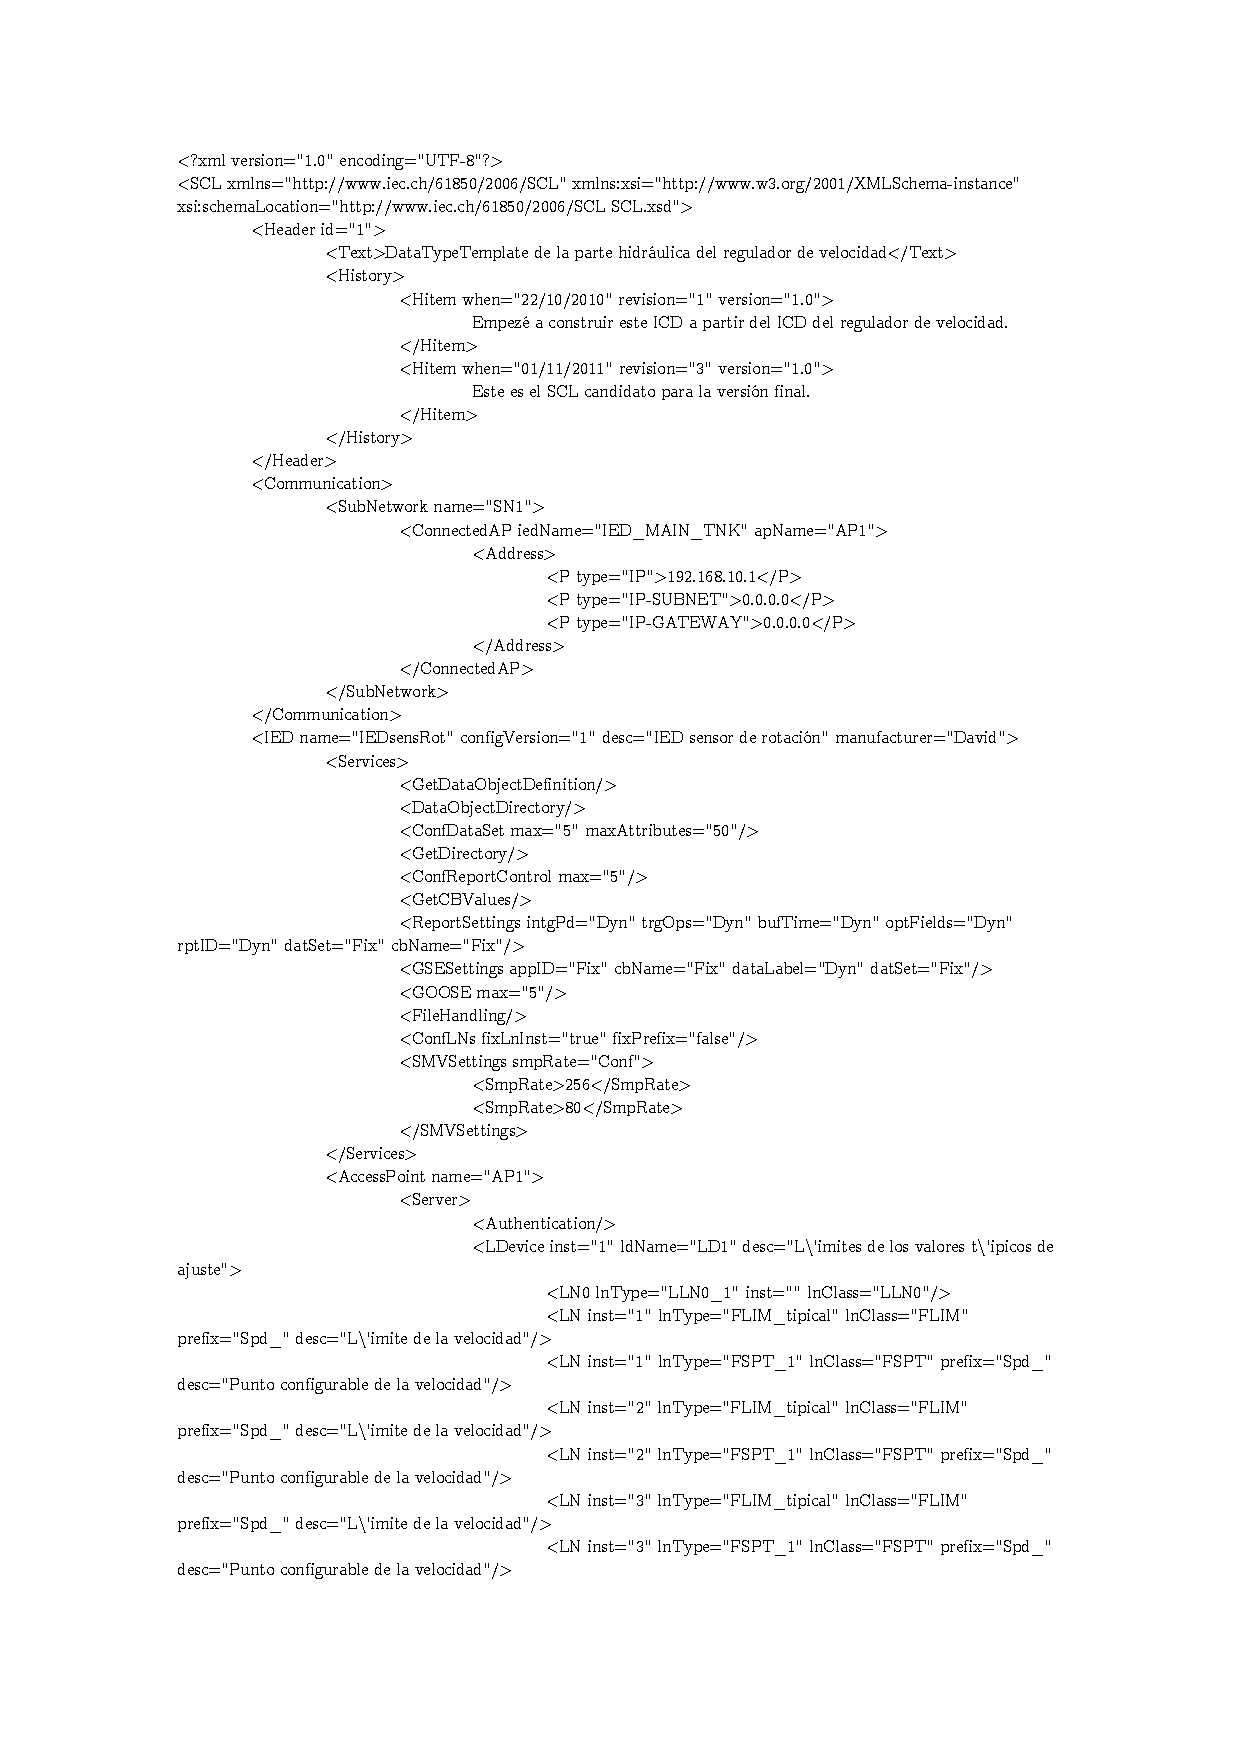
\includepdf[pages=1-4]{appendices/ICD-IED_rot_sensor.pdf} 


\vspace*{\fill}
	\begingroup
\section{ICD del tanque principal}
	\endgroup
\vspace*{\fill}
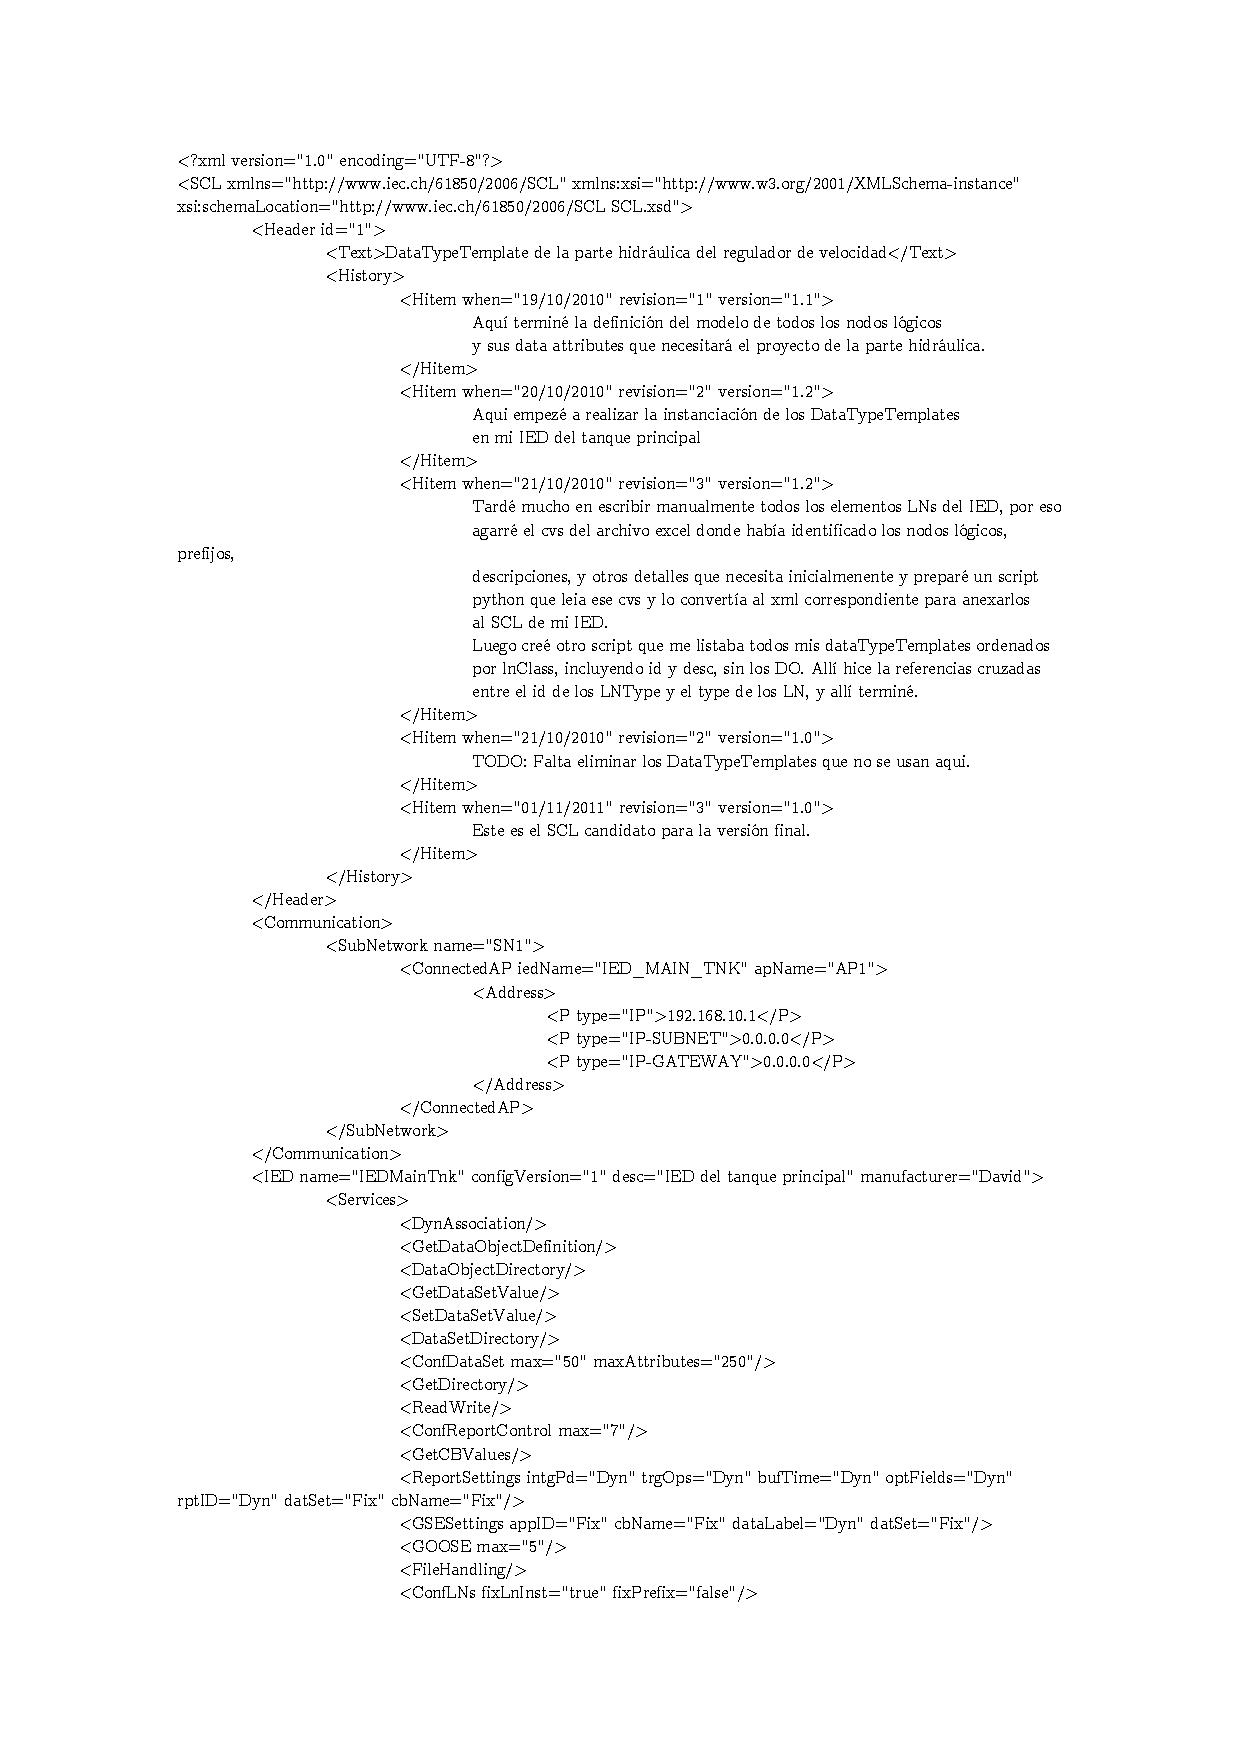
\includepdf[pages=1-11]{appendices/ICD-IED_MAIN_TNK.pdf} 



\vspace*{\fill}
	\begingroup
\section{ICD de la planta a aire comprimido}
	\endgroup
\vspace*{\fill}
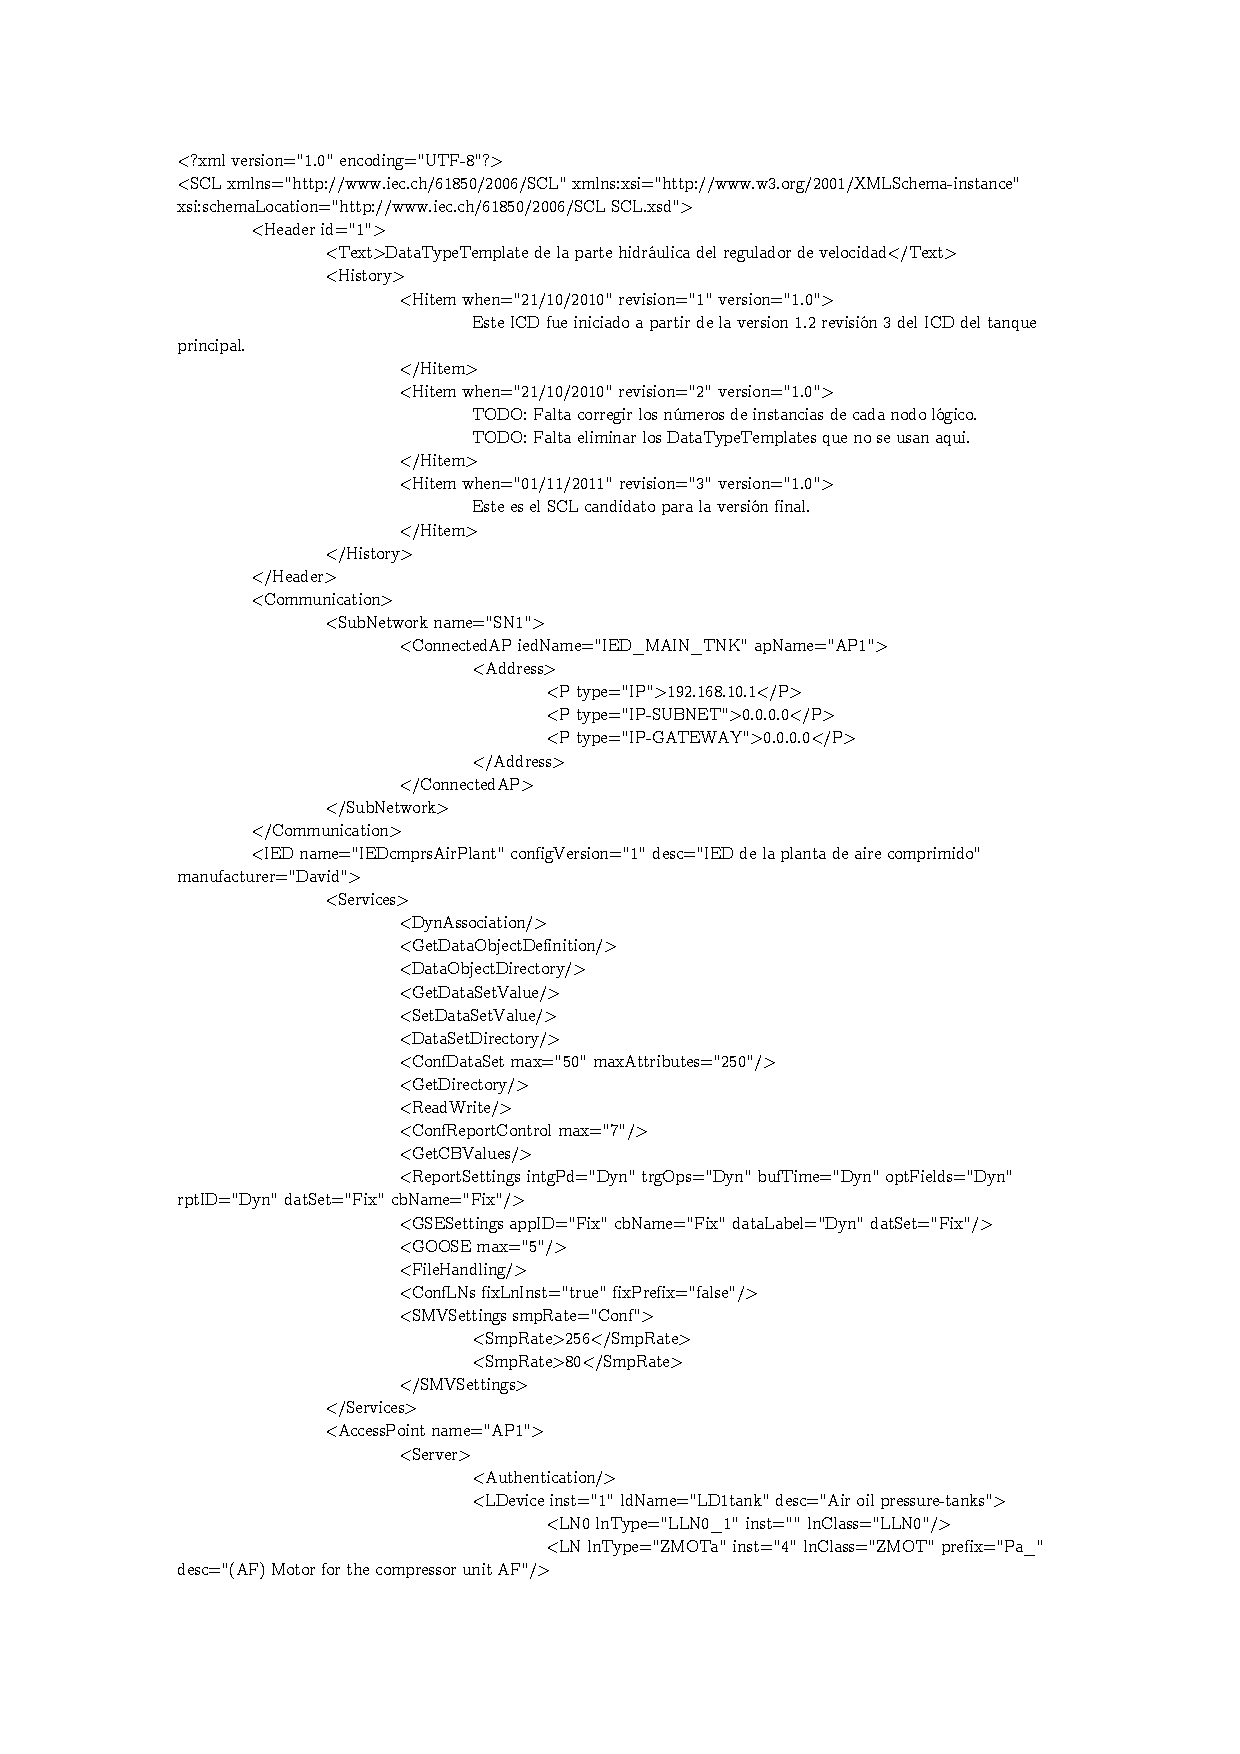
\includepdf[pages=1-4]{appendices/ICD-IED_compressed_air_plant.pdf} 



\vspace*{\fill}
	\begingroup
\section{ICD del tanque de compresi�n de aire y de aceite}
	\endgroup
\vspace*{\fill}
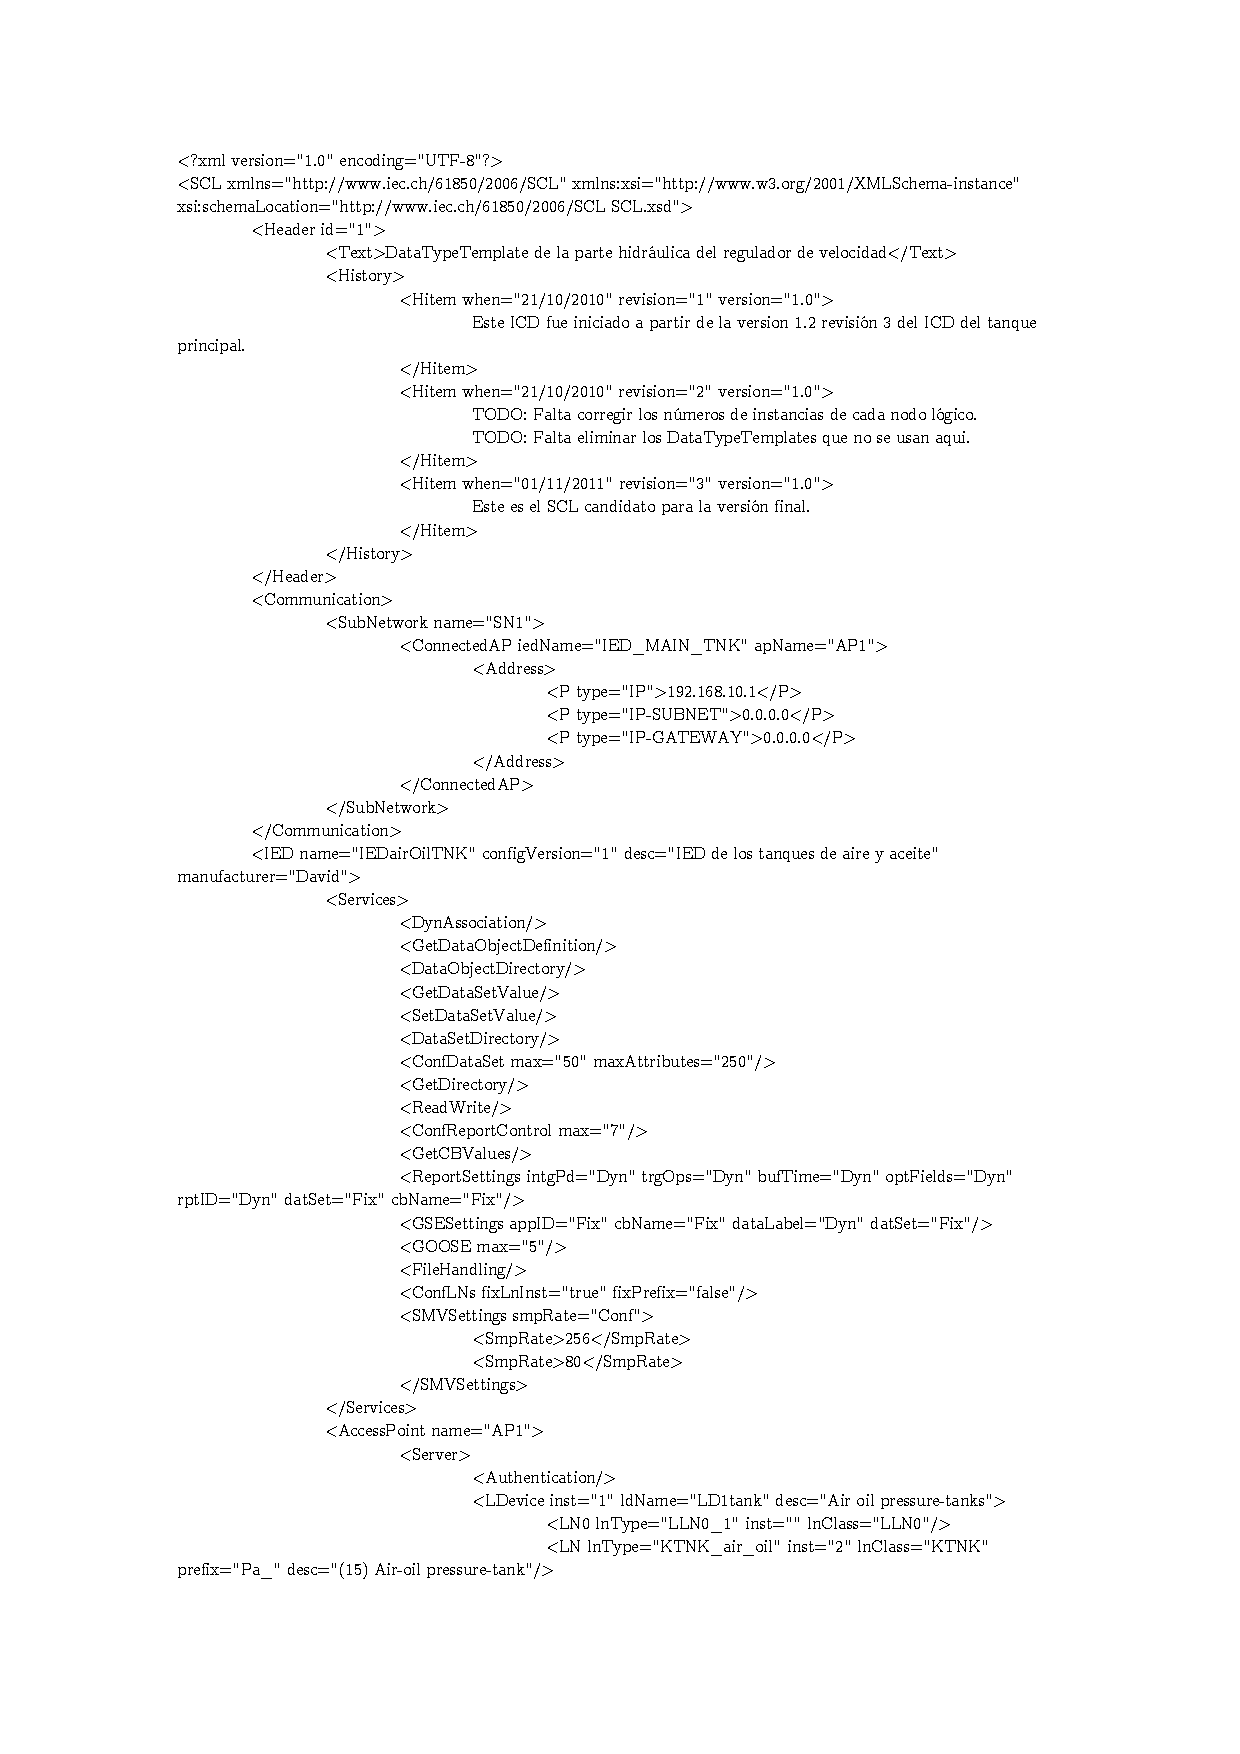
\includepdf[pages=1-6]{appendices/ICD-IED_air-oil_PRS_TNK.pdf} 
  



\vspace*{\fill}
	\begingroup
\section{SSD de todo el sistema}
	\endgroup
\vspace*{\fill}
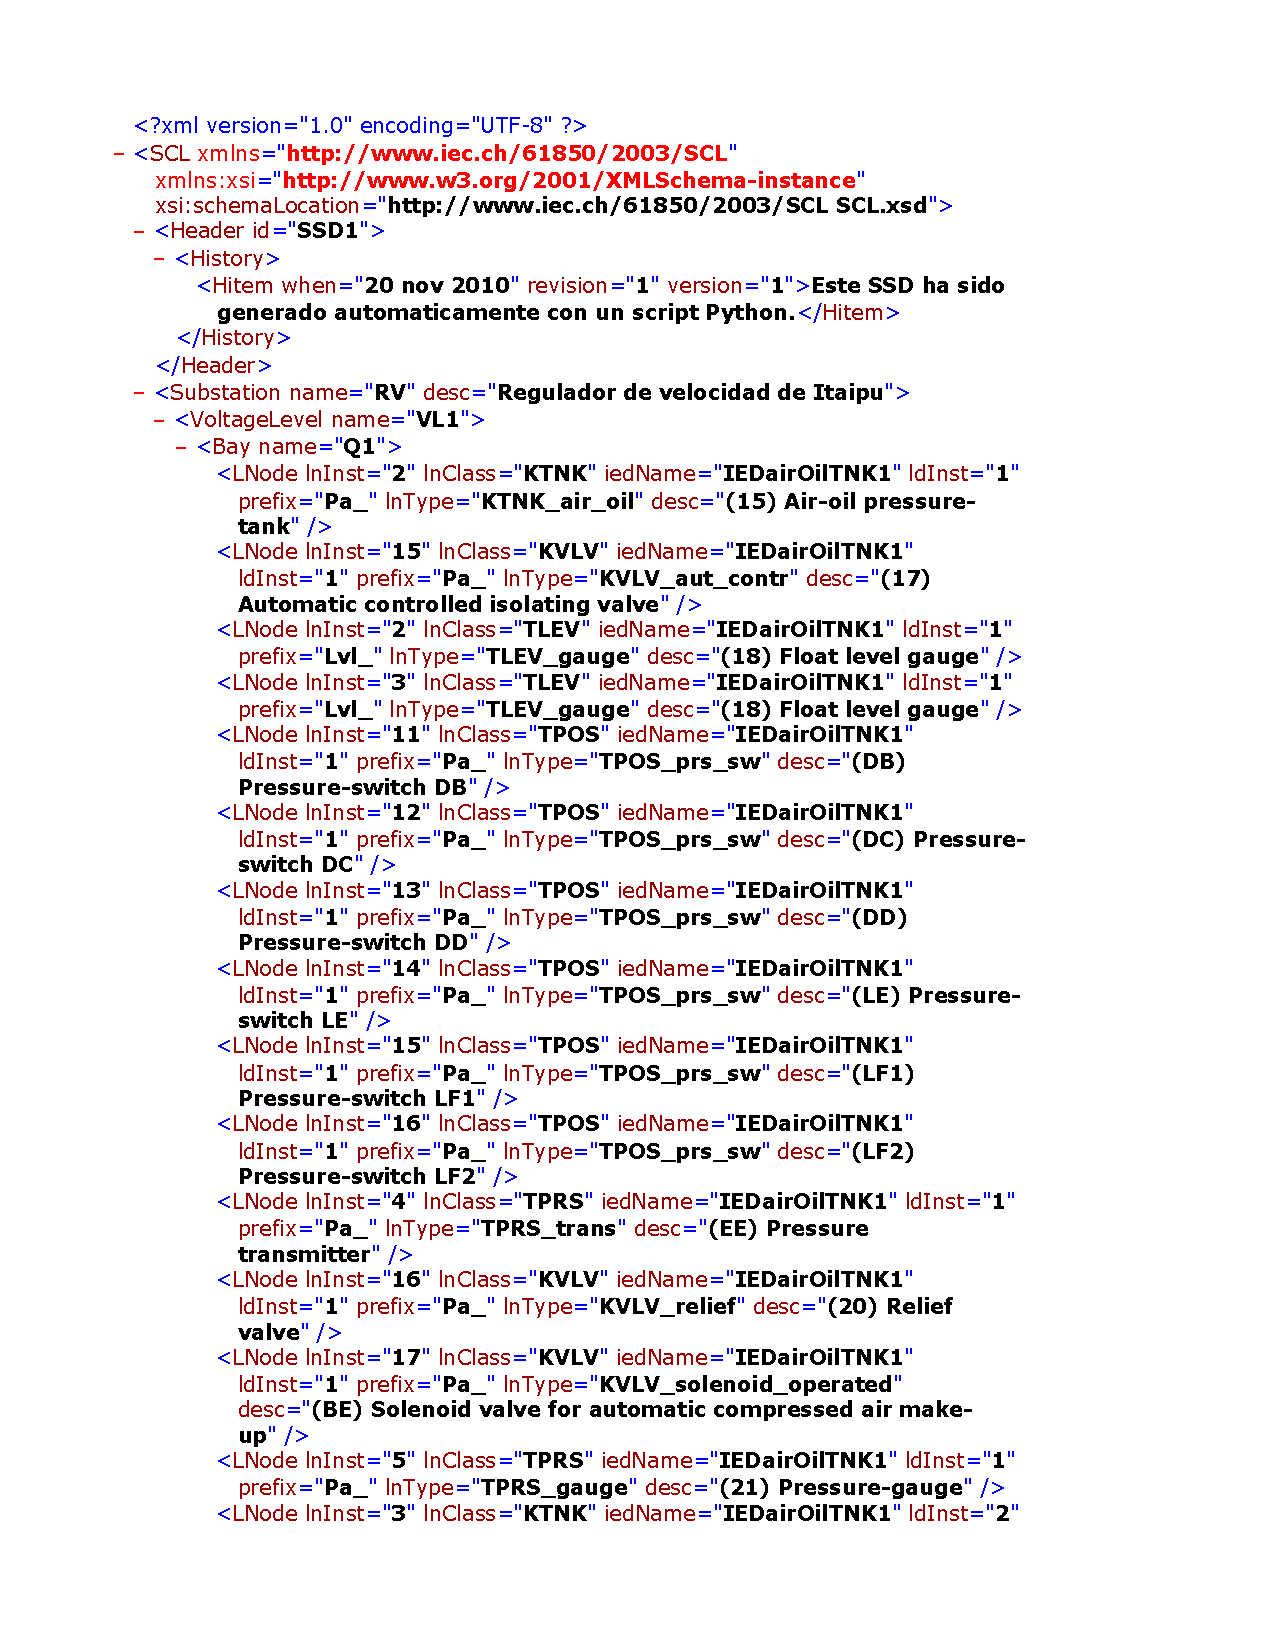
\includepdf[pages=1-21]{appendices/SSD_MRV.pdf} 
  
  
 
\section{SCL XML Shemas modificados asociados a los ICDs del proyecto}

Para este trabajo se han utilizado los XML Shemas 
definidos en el apartado IEC 61850-6, edici�n 1 \cite{IEC61850-6:2004},
y se han realizado algunas modificaciones, 
proveidas en las secciones los c�digos fuente \ref{cod:scl-xsd} y
\ref{cod:SCL_Enums-xsd}, para agregar los nodos l�gicos 
para centrales hidroel�ctricas 
definidos en IEC 61850-7-410 \cite{IEC61850-7-410:2007}. En 
los dem�s ficheros \emph{XSD} s�lo se ha modificado
el espacio de nombres, que originalmente estaba
definido con la URL de 2006 en \cite{IEC61850-6:2004},
y en el presente trabajo se cambi� dicho espacio 
de nombres para la URL de 2003 de la iec, 
porque el la herramienta de ingenier�a Atlan61850
s�lo aceptaba este espacio de nombres. Con la herramienta
Atlan61850 fue obtenida la figura \ref{fig:LNodes-reg-veloc}
(y luego han sido retocados con otro software de prop�sito general 
para la edici�n de im�genes).

Est� claro que 
utilizar el fichero XSD 
\emph{SCL\_Maintenance} para 
realizar estas modificaciones
es una buena pr�ctica. Dicho 
enfoque ser� considerado por el autor para un 
trabajo futuro (los resultados son los mismos,
s�lo cambia la modularidad del c�digo fuente 
donde se encuentran las definciones).

	\subsection{SCL.xsd}
		\lstinputlisting[label=cod:scl-xsd,
		caption=SCL.xsd]
		{governorModel/xsd2003/SCL.xsd} 

	\subsection{SCL\_Enums.xsd}
		\lstinputlisting[label=cod:SCL_Enums-xsd,
		caption=SCL\_Enums.xsd]
		{governorModel/xsd2003/SCL_Enums.xsd} 

